% Options for packages loaded elsewhere
\PassOptionsToPackage{unicode}{hyperref}
\PassOptionsToPackage{hyphens}{url}
%
\documentclass[
  letterpaper,
]{scrbook}

\usepackage{amsmath,amssymb}
\usepackage{iftex}
\ifPDFTeX
  \usepackage[T1]{fontenc}
  \usepackage[utf8]{inputenc}
  \usepackage{textcomp} % provide euro and other symbols
\else % if luatex or xetex
  \usepackage{unicode-math}
  \defaultfontfeatures{Scale=MatchLowercase}
  \defaultfontfeatures[\rmfamily]{Ligatures=TeX,Scale=1}
\fi
\usepackage[]{libertinus}
\ifPDFTeX\else  
    % xetex/luatex font selection
\fi
% Use upquote if available, for straight quotes in verbatim environments
\IfFileExists{upquote.sty}{\usepackage{upquote}}{}
\IfFileExists{microtype.sty}{% use microtype if available
  \usepackage[]{microtype}
  \UseMicrotypeSet[protrusion]{basicmath} % disable protrusion for tt fonts
}{}
\makeatletter
\@ifundefined{KOMAClassName}{% if non-KOMA class
  \IfFileExists{parskip.sty}{%
    \usepackage{parskip}
  }{% else
    \setlength{\parindent}{0pt}
    \setlength{\parskip}{6pt plus 2pt minus 1pt}}
}{% if KOMA class
  \KOMAoptions{parskip=half}}
\makeatother
\usepackage{xcolor}
\setlength{\emergencystretch}{3em} % prevent overfull lines
\setcounter{secnumdepth}{5}
% Make \paragraph and \subparagraph free-standing
\ifx\paragraph\undefined\else
  \let\oldparagraph\paragraph
  \renewcommand{\paragraph}[1]{\oldparagraph{#1}\mbox{}}
\fi
\ifx\subparagraph\undefined\else
  \let\oldsubparagraph\subparagraph
  \renewcommand{\subparagraph}[1]{\oldsubparagraph{#1}\mbox{}}
\fi


\providecommand{\tightlist}{%
  \setlength{\itemsep}{0pt}\setlength{\parskip}{0pt}}\usepackage{longtable,booktabs,array}
\usepackage{calc} % for calculating minipage widths
% Correct order of tables after \paragraph or \subparagraph
\usepackage{etoolbox}
\makeatletter
\patchcmd\longtable{\par}{\if@noskipsec\mbox{}\fi\par}{}{}
\makeatother
% Allow footnotes in longtable head/foot
\IfFileExists{footnotehyper.sty}{\usepackage{footnotehyper}}{\usepackage{footnote}}
\makesavenoteenv{longtable}
\usepackage{graphicx}
\makeatletter
\def\maxwidth{\ifdim\Gin@nat@width>\linewidth\linewidth\else\Gin@nat@width\fi}
\def\maxheight{\ifdim\Gin@nat@height>\textheight\textheight\else\Gin@nat@height\fi}
\makeatother
% Scale images if necessary, so that they will not overflow the page
% margins by default, and it is still possible to overwrite the defaults
% using explicit options in \includegraphics[width, height, ...]{}
\setkeys{Gin}{width=\maxwidth,height=\maxheight,keepaspectratio}
% Set default figure placement to htbp
\makeatletter
\def\fps@figure{htbp}
\makeatother
\newlength{\cslhangindent}
\setlength{\cslhangindent}{1.5em}
\newlength{\csllabelwidth}
\setlength{\csllabelwidth}{3em}
\newlength{\cslentryspacingunit} % times entry-spacing
\setlength{\cslentryspacingunit}{\parskip}
\newenvironment{CSLReferences}[2] % #1 hanging-ident, #2 entry spacing
 {% don't indent paragraphs
  \setlength{\parindent}{0pt}
  % turn on hanging indent if param 1 is 1
  \ifodd #1
  \let\oldpar\par
  \def\par{\hangindent=\cslhangindent\oldpar}
  \fi
  % set entry spacing
  \setlength{\parskip}{#2\cslentryspacingunit}
 }%
 {}
\usepackage{calc}
\newcommand{\CSLBlock}[1]{#1\hfill\break}
\newcommand{\CSLLeftMargin}[1]{\parbox[t]{\csllabelwidth}{#1}}
\newcommand{\CSLRightInline}[1]{\parbox[t]{\linewidth - \csllabelwidth}{#1}\break}
\newcommand{\CSLIndent}[1]{\hspace{\cslhangindent}#1}

<script src="site_libs/htmlwidgets-1.6.2/htmlwidgets.js"></script>
<link href="site_libs/datatables-css-0.0.0/datatables-crosstalk.css" rel="stylesheet" />
<script src="site_libs/datatables-binding-0.28/datatables.js"></script>
<script src="site_libs/jquery-3.6.0/jquery-3.6.0.min.js"></script>
<link href="site_libs/dt-core-1.13.4/css/jquery.dataTables.min.css" rel="stylesheet" />
<link href="site_libs/dt-core-1.13.4/css/jquery.dataTables.extra.css" rel="stylesheet" />
<script src="site_libs/dt-core-1.13.4/js/jquery.dataTables.min.js"></script>
<link href="site_libs/crosstalk-1.2.0/css/crosstalk.min.css" rel="stylesheet" />
<script src="site_libs/crosstalk-1.2.0/js/crosstalk.min.js"></script>
\makeatletter
\makeatother
\makeatletter
\@ifpackageloaded{bookmark}{}{\usepackage{bookmark}}
\makeatother
\makeatletter
\@ifpackageloaded{caption}{}{\usepackage{caption}}
\AtBeginDocument{%
\ifdefined\contentsname
  \renewcommand*\contentsname{Table of contents}
\else
  \newcommand\contentsname{Table of contents}
\fi
\ifdefined\listfigurename
  \renewcommand*\listfigurename{List of Figures}
\else
  \newcommand\listfigurename{List of Figures}
\fi
\ifdefined\listtablename
  \renewcommand*\listtablename{List of Tables}
\else
  \newcommand\listtablename{List of Tables}
\fi
\ifdefined\figurename
  \renewcommand*\figurename{Figure}
\else
  \newcommand\figurename{Figure}
\fi
\ifdefined\tablename
  \renewcommand*\tablename{Table}
\else
  \newcommand\tablename{Table}
\fi
}
\@ifpackageloaded{float}{}{\usepackage{float}}
\floatstyle{ruled}
\@ifundefined{c@chapter}{\newfloat{codelisting}{h}{lop}}{\newfloat{codelisting}{h}{lop}[chapter]}
\floatname{codelisting}{Listing}
\newcommand*\listoflistings{\listof{codelisting}{List of Listings}}
\makeatother
\makeatletter
\@ifpackageloaded{caption}{}{\usepackage{caption}}
\@ifpackageloaded{subcaption}{}{\usepackage{subcaption}}
\makeatother
\makeatletter
\@ifpackageloaded{tcolorbox}{}{\usepackage[skins,breakable]{tcolorbox}}
\makeatother
\makeatletter
\@ifundefined{shadecolor}{\definecolor{shadecolor}{rgb}{.97, .97, .97}}
\makeatother
\makeatletter
\makeatother
\makeatletter
\makeatother
\ifLuaTeX
  \usepackage{selnolig}  % disable illegal ligatures
\fi
\IfFileExists{bookmark.sty}{\usepackage{bookmark}}{\usepackage{hyperref}}
\IfFileExists{xurl.sty}{\usepackage{xurl}}{} % add URL line breaks if available
\urlstyle{same} % disable monospaced font for URLs
\hypersetup{
  pdftitle={Statistics 1 and 2},
  pdfauthor={Caspar J. Van Lissa},
  hidelinks,
  pdfcreator={LaTeX via pandoc}}

\title{Statistics 1 and 2}
\author{Caspar J. Van Lissa}
\date{}

\begin{document}
\frontmatter
\maketitle
\ifdefined\Shaded\renewenvironment{Shaded}{\begin{tcolorbox}[sharp corners, frame hidden, boxrule=0pt, interior hidden, borderline west={3pt}{0pt}{shadecolor}, breakable, enhanced]}{\end{tcolorbox}}\fi

\renewcommand*\contentsname{Table of contents}
{
\setcounter{tocdepth}{2}
\tableofcontents
}
\mainmatter
\bookmarksetup{startatroot}

\hypertarget{overview}{%
\chapter*{Overview}\label{overview}}
\addcontentsline{toc}{chapter}{Overview}

\markboth{Overview}{Overview}

This course covers the basics of statistics and data analysis. The
ability to extract insights from data is an essential skill for both
academic and non-academic work, and ``data literacy'' is increasingly
important in a world where data are collected about every aspect of our
lives. After completing this course, you will be able to independently
analyze data, interpret and report your findings, and assess the results
of analyses performed by others, such as you might find in scientific
articles.

This GitBook contains all relevant information about this course. It is
assumed that every student reads it carefully. If you have any
questions, first consult this GitBook, then ask a fellow student, and
only if your question is still not answered, then contact the course
coordinator.

Communication about the course occurs through Canvas (Login with your
student ID and password).

\hypertarget{course-overview}{%
\section*{Course overview}\label{course-overview}}
\addcontentsline{toc}{section}{Course overview}

\markright{Course overview}

The \textbf{course schedule} is available on Osiris. For an overview of
the content, see below:

\begin{verbatim}
Warning: package 'DT' was built under R version 4.3.1
\end{verbatim}

\hypertarget{literature-software}{%
\section*{Literature \& Software}\label{literature-software}}
\addcontentsline{toc}{section}{Literature \& Software}

\markright{Literature \& Software}

\textbf{You do not need a book for this course!}

All essential information is contained within this GitBook.

During lab sessions, you work on the exercises and your portfolio using
the commercial SPSS software installed on university computers.

If you want to use your own computer instead, you might consider trying
some free alternatives to SPSS:

\begin{itemize}
\tightlist
\item
  PSPP, which is designed to be nearly identical to SPSS with all the
  same basic functionality: https://www.gnu.org/software/pspp/pspp.html
\item
  JASP, which is more modern, looks nicer and is very easy to use -- but
  looks less similar to SPSS: https://jasp-stats.org/
\end{itemize}

\hypertarget{learning-goals}{%
\section*{Learning goals}\label{learning-goals}}
\addcontentsline{toc}{section}{Learning goals}

\markright{Learning goals}

After taking this course, students will be able to\ldots{}

\hypertarget{all-majors}{%
\subsection*{All majors}\label{all-majors}}
\addcontentsline{toc}{subsection}{All majors}

\begin{enumerate}
\def\labelenumi{\arabic{enumi}.}
\tightlist
\item
  compute and interpret commonly used descriptive statistics such as the
  sample mean, the median, the mode, variance and standard deviation,
  the standard error, and the correlation coefficient.
\item
  recognize different probability distributions such as the normal
  distribution, and make computations for these probability
  distributions.
\item
  explain the essential aspects of null-hypothesis significance testing,
  including sampling distributions, Type I and Type II errors,
  one-tailed versus two-tailed testing, and statistical power.
\item
  apply different statistical tests such as the Z-test, the one sample
  t-test, the one way Between Subjects Analysis of Variance test, and
  statistical tests related to (multiple) linear regression analysis
  with continuous and categorical predictors; and clarify the
  statistical and/or methodological assumptions that apply to the
  techniques that are discussed in this course.
\item
  explain basic concepts in regression analysis, including: linear
  association, least-squares estimation, explained variance, Multiple R,
  multiple correlation, adjusted R-square, raw and standardized
  regression coefficients, model-comparison tests, predicted scores,
  residuals and the assumptions;
\item
  choose the appropriate analysis technique for answering a specific
  research problem from the range of techniques that are covered in the
  course.
\item
  use the software package SPSS to perform several statistical data
  analyses and be able to correctly interpret and report the output to
  an informed audience (e.g., Liberal arts students, researchers from
  the social sciences/business and economics/cognitive neuroscience).
\item
  draw valid conclusions from the results of empirical data analyses
  given specific research questions envisaged.
\end{enumerate}

\hypertarget{major-business-and-economics}{%
\subsection*{Major Business and
Economics}\label{major-business-and-economics}}
\addcontentsline{toc}{subsection}{Major Business and Economics}

\begin{enumerate}
\def\labelenumi{\arabic{enumi}.}
\setcounter{enumi}{8}
\tightlist
\item
  apply statistical tests in the context of multiple linear regression
  models with interaction terms and logistic regression models;
  interpret the corresponding output.
\item
  describe the concepts of probabilities, odds and logits; describe the
  relationship between the three scales; transform one into another
  (formulae are provided).
\end{enumerate}

\hypertarget{major-cognitive-neuroscience}{%
\subsection*{Major Cognitive
Neuroscience}\label{major-cognitive-neuroscience}}
\addcontentsline{toc}{subsection}{Major Cognitive Neuroscience}

\begin{enumerate}
\def\labelenumi{\arabic{enumi}.}
\setcounter{enumi}{10}
\tightlist
\item
  apply statistical tests in the context of factorial ANOVA, ANCOVA and
  Analysis of Repeated measures; interpret the corresponding output; and
  calculate and interpret effect size estimates relevant for these
  statistical techniques (e.g., (partial) eta squared)
\end{enumerate}

\hypertarget{major-social-sciences}{%
\subsection*{Major Social Sciences}\label{major-social-sciences}}
\addcontentsline{toc}{subsection}{Major Social Sciences}

\begin{enumerate}
\def\labelenumi{\arabic{enumi}.}
\setcounter{enumi}{11}
\tightlist
\item
  apply statistical tests in the context of multiple linear regression
  models with interaction terms and interpret the corresponding output.
\item
  gauge the reliability of measurements from questionnaires and identify
  problematic items.
\item
  explore the dimensionality of questionnaire data.
\end{enumerate}

\hypertarget{attendance}{%
\section*{Attendance}\label{attendance}}
\addcontentsline{toc}{section}{Attendance}

\markright{Attendance}

Attendance is mandatory based on our experience that students who
actively participate tend to pass the course, whereas those who do not
tend to drop out or fail. All lectures and practicals `build' on each
other, so if you have to miss either one, absolutely make sure you have
caught up with the materials before the next session.

\hypertarget{staff}{%
\section*{Staff}\label{staff}}
\addcontentsline{toc}{section}{Staff}

\markright{Staff}

\textbf{Coordinator:}

\href{https://www.tilburguniversity.edu/nl/medewerkers/c-j-vanlissa}{dr.
Caspar J. van Lissa}

\textbf{Lab sessions}

(Thu) Tra Lê

\hypertarget{teaching-philosophy}{%
\section*{Teaching Philosophy}\label{teaching-philosophy}}
\addcontentsline{toc}{section}{Teaching Philosophy}

\markright{Teaching Philosophy}

The corona crisis is challenging all of us to rethink how we teach and
learn. But aside from the challenges, it also offers opportunities. In
adapting this course, we kept two goals in mind: increasing the
alignment between the way of teaching and the learning goals, and
ensuring high-quality interaction among students and between the
students and teachers while still using online communication. Based on
these goals, we made the following changes:

\begin{enumerate}
\def\labelenumi{\arabic{enumi}.}
\tightlist
\item
  During the course, you will be working in learning teams to promote
  interaction among students and peer support
\item
  The two in-person exams (4 hours each) are replaced with take-home
  assignments: Two group assignments, and one individual assignment.
\end{enumerate}

\hypertarget{why-group-assignments}{%
\subsection*{Why group assignments?}\label{why-group-assignments}}
\addcontentsline{toc}{subsection}{Why group assignments?}

Contact with fellow students is a key aspect of the university
experience. We want to stimulate you to engage with the material and
with one another. Therefore, the portfolio assignments are made in
groups. There are also aspects of learning in groups that can really
improve your knowledge, like peer feedback. To ensure that every group
member pulls their weight, the final exam tests each student's
individual comprehension of all material covered in the portfolios.

Groups comprise 3-5 members and are assigned randomly when the course
starts. However, it is allowed to switch with a consenting member of
another group, or to join/merge with another small group if your group
has become smaller than 3 members. There are three portfolio
registration deadlines. At this point, one group member submits the
definitive group composition via a Google form.

\hypertarget{why-use-portfolio-assessment}{%
\subsection*{Why use portfolio
assessment?}\label{why-use-portfolio-assessment}}
\addcontentsline{toc}{subsection}{Why use portfolio assessment?}

Portfolio assignments are well-suited for a skills-based course like
Statistics 1 \& 2. They also take a lot of the pressure off because you
can work at your own pace, and keep improving the work until it is good
enough. We entrust you with the responsibility of making these portfolio
assignments in good faith, without instrumental assistance from outside
your group or plagiarism, so I kindly ask you to make good on this
trust, and hand in original work to show what you've learned.

\hypertarget{use-of-ai-for-making-assignments}{%
\subsection*{Use of AI for making
assignments}\label{use-of-ai-for-making-assignments}}
\addcontentsline{toc}{subsection}{Use of AI for making assignments}

There is, in principle, nothing wrong with using AI-based tools like
ChatGPT, as you will also have access to them in your working life - but
be warned: when you use ChatGPT, it is your responsibility to thoroughly
check its output for logical consistency and correctness. You may not
yet have the level of expertise required to know when ChatGPT generates
irrelevant nonsense - but the teacher who grades your work does.
Consider this carefully when deciding what makes more sense: doing your
work manually, making sure each step is correct - or outsourcing it to
AI, and then checking its work before submitting.

\hypertarget{grading}{%
\section*{Grading}\label{grading}}
\addcontentsline{toc}{section}{Grading}

\markright{Grading}

Your grade is based on three portfolio assignments made in groups, and
one individual exam to test comprehension of the material covered in the
portfolios.

\hypertarget{portfolios-40-3-x-13.3}{%
\subsection*{Portfolios 40\% (3 x
13.3\%)}\label{portfolios-40-3-x-13.3}}
\addcontentsline{toc}{subsection}{Portfolios 40\% (3 x 13.3\%)}

You work on the portfolio assignments with your group, both during the
lab sessions and outside of class. You hand in your group's portfolio
assignment before the set deadline, at which point it is graded. If your
grade is below the passing level of 5.5, your group will have the
opportunity to revise the portfolio based on teacher feedback to receive
a maximum grade of 6.

\hypertarget{exam-60}\label{exam-60}}
\addcontentsline{toc}{subsection}{Exam 60\%}

To make sure that all students are equally involved in the making of the
portfolio assignments, an individual exam assesses comprehension of the
material covered therein. It is a digital multiple choice exam. You may
bring all course materials to the exam, including the portfolio. The
exam consists of a common part and a major-specific part. Note: As per
university policy, a guessing correction is applied to your grade.

\hypertarget{assignments}{%
\section*{Assignments}\label{assignments}}
\addcontentsline{toc}{section}{Assignments}

\markright{Assignments}

A description of the assignments follows below. For each assignment,
every element labeled with a lower case letter is graded fail (0
points), pass (1 point), or excellent (1.5 points). Grades are summed
for each assignment, and rescaled from 1-10. The final grade is a
weighted average across assignments of the rescaled grades (weights in
\%). Note that the assignments are \textbf{not} full-length papers! You
only get 200 words to justify your theoretical model, and 300 words to
discuss the results. The focus should be on your analysis; how it
relates to theory (introduction), and what you have learned from it and
how you might improve it (discussion).

\begin{enumerate}
\def\labelenumi{\arabic{enumi}.}
\tightlist
\item
  Apply the ``latent variable model'' to a real-life problem, where
  observed variables do not directly measure, but are indicators of, an
  unobserved social scientific construct (G, 25\%)

  \begin{enumerate}
  \def\labelenumii{\alph{enumii}.}
  \tightlist
  \item
    Find a suitable dataset, for example: (no word limit)

    \begin{enumerate}
    \def\labelenumiii{\roman{enumiii}.}
    \tightlist
    \item
      Data you have collected for a previous course
    \item
      Open data, provided with a published paper
    \item
      The ``Coping with COVID-19'' dataset (if you can't find anything)
    \end{enumerate}
  \item
    Describe the dataset, and introduce the theoretical latent variable
    model (200 words)
  \item
    Estimate the latent variable model (PCA, EFA, CFA) and conduct
    reliability analysis, provide relevant output in a suitable format
    (no word limit; as short as possible and as long as necessary to
    report the relevant output)
  \item
    Explain your rationale for important modeling decisions (300 words)

    \begin{enumerate}
    \def\labelenumiii{\roman{enumiii}.}
    \tightlist
    \item
      Motivate your choice for the type of latent variable model
    \item
      Discuss assumptions
    \item
      Discuss other important decisions, as discussed in the course
      reading materials
    \end{enumerate}
  \item
    Report and interpret the results in APA style (no word limit; as
    short as possible and as long as necessary to report the relevant
    results)
  \item
    Discuss the results in max 300 words

    \begin{enumerate}
    \def\labelenumiii{\roman{enumiii}.}
    \tightlist
    \item
      Devote attention to strengths and limitations
    \end{enumerate}
  \end{enumerate}
\item
  Use the ``path model'' to describe how several variables are causally
  related to one another (G, 25\%)

  \begin{enumerate}
  \def\labelenumii{\alph{enumii}.}
  \tightlist
  \item
    Find a suitable dataset, for example: (no word limit)

    \begin{enumerate}
    \def\labelenumiii{\roman{enumiii}.}
    \tightlist
    \item
      Data you have collected and analyzed for a previous course
    \item
      Open data, provided with a published paper
    \item
      The ``Coping with COVID-19'' dataset (if you can't find anything)
    \end{enumerate}
  \item
    Describe the dataset, and introduce the theoretical path model (200
    words)
  \item
    Conduct a SEM path model to answer the theoretical questions (no
    word limit; as short as possible and as long as necessary to report
    the relevant output)

    \begin{enumerate}
    \def\labelenumiii{\roman{enumiii}.}
    \tightlist
    \item
      This can be a re-analysis of a question that had been tested using
      regression, ANOVA, or t-test analysis in the original paper
    \end{enumerate}
  \item
    Explain your rationale for important modeling decisions (300 words)

    \begin{enumerate}
    \def\labelenumiii{\roman{enumiii}.}
    \tightlist
    \item
      Fit between theory and model
    \item
      Model assumptions
    \item
      Difference/similarity between the path model and the (original)
      regression, ANOVA, or t-test analysis
    \item
      Why you use standardized or unstandardized coefficients
    \end{enumerate}
  \item
    Report and interpret the results in APA style (no word limit; as
    short as possible and as long as necessary to report the relevant
    results)

    \begin{enumerate}
    \def\labelenumiii{\roman{enumiii}.}
    \tightlist
    \item
      Include measures of explained variance for the dependent
      variables.
    \end{enumerate}
  \item
    Discuss the results (max 300 words)

    \begin{enumerate}
    \def\labelenumiii{\roman{enumiii}.}
    \tightlist
    \item
      Devote attention to strengths and limitations
    \end{enumerate}
  \end{enumerate}
\item
  Independently analyze data using the free, open-source statistical
  software R (I, 50\%)

  \begin{enumerate}
  \def\labelenumii{\alph{enumii}.}
  \tightlist
  \item
    Find a suitable dataset, for example: (no word limit)

    \begin{enumerate}
    \def\labelenumiii{\roman{enumiii}.}
    \tightlist
    \item
      Data you have collected for a previous course
    \item
      Open data, provided with a published paper
    \item
      The ``Coping with COVID-19'' dataset (if you can't find anything)
    \end{enumerate}
  \item
    Describe the dataset, and introduce a theory involving at least 3
    variables that can be tested using these data (300 words)
  \item
    Translate the theory to lavaan syntax and estimate the model (could
    be multiple models if you think it's necessary; no word limit)
  \item
    Use at least all of the following: (no word limit)

    \begin{enumerate}
    \def\labelenumiii{\roman{enumiii}.}
    \tightlist
    \item
      One latent variable
    \item
      Moderation (continuous or multi-group)
    \item
      Mediation
    \end{enumerate}
  \item
    Explain your rationale for important modeling decisions (300 words)

    \begin{enumerate}
    \def\labelenumiii{\roman{enumiii}.}
    \tightlist
    \item
      Fit between theory and model
    \item
      Model assumptions
    \item
      Difference/similarity between the path model and the (original)
      regression, ANOVA, or t-test analysis
    \item
      Why you use standardized or unstandardized coefficients
    \end{enumerate}
  \item
    Report and interpret your results in APA style (no word limit; as
    short as possible and as long as necessary to report the relevant
    results)
  \item
    Discuss your results in maximum 500 words
  \end{enumerate}
\end{enumerate}

\hypertarget{credit}{%
\section*{Credit}\label{credit}}
\addcontentsline{toc}{section}{Credit}

\markright{Credit}

This book is based on Lisa DeBruine's ``booktem'':

\begin{quote}
DeBruine L, Lakens D (2023). \emph{booktem: Methods Book Template}.
https://github.com/debruine/booktem,
https://debruine.github.io/booktem/.
\end{quote}

Also see: https://psyteachr.github.io/

\bookmarksetup{startatroot}

\hypertarget{sec-intro}{%
\chapter{Introduction to Statistics}\label{sec-intro}}

Statistics are more relevant than ever in this digital age, where data
about our entire lives is readily available, and software to analyze
such data has become extremely user-friendly and freely available. We
live in a world where everyone wants our data, and being data literate
is becoming increasingly important across industries.

Statistics allows us to make sense of data and gain valuable insights.
It helps us better understand social phenomena, predict sales and
optimize marketing strategies, and even explore the relationship between
brain activity and behavior. Data analysis is one of the most marketable
skills taught at universities.

Before we delve deeper into statistics, it's crucial to distinguish
between methods and statistics. Methods refer to the procedures used in
research, such as data collection, participant selection, and study
design. On the other hand, statistics focuses on analyzing the data
obtained from these methods.

Two fundamental branches of statistics covered in this course are
descriptive statistics and inferential statistics. Descriptive
statistics involves summarizing and describing the characteristics of a
dataset, while inferential statistics allows us to make educated guesses
about a larger population based on a smaller sample.

Statistical modeling is another aspect of statistics where theories are
represented mathematically. This enables us to predict important
outcomes, such as sales figures, well-being, or the likelihood of
neurological disorders. Statistical modeling also allows us to explore
data for interesting patterns or to perform tests to answer
theoretically driven research questions.

In scientific research, statistics can help us test theories. The
process of scientific knowledge acquisition is described by the
empirical cycle: We start with a theory, from which we derive testable
hypotheses. A theory is an abstract system of assumptions about the
relationships between constructs. A hypothesis is a concrete statement,
derived from the theory, about expected quantitative relationships
between measured variables. We then collect data and test the
hypothesis. If the hypothesis is refuted, we re-examine the theory and
possibly ammend it.

To lay a foundation for understanding statistics, it's essential to be
familiar with some basic concepts. First, data in the social sciences
often comes in tabular format (e.g., spreadsheets), where each row
represents an individual observation, and each column represents the
individuals' scores on various variables.

A crucial distinction is the one between population and sample. The
population refers to the complete set of objects of interest, such as
all people in a country or all students in a class. However, due to
practical limitations, we usually do not have access to the population.
Instead, we draw a sample from it, which is a subset of the population.
Sampling theory establishes the rationale for drawing inferences about a
population based on samples. Sample statistics serve as our best
estimate of population parameters. If the sample is representative,
those estimates will be unbiased. Moreover, we can estimate our
uncertainty about the sample statistics as estimates of population
parameters. The best way to ensure a representative sample is to use
random sampling, where each individual in the population has an equal
chance of being included.

The distinction between constructs and variables is also important.
Constructs are abstract features of interest within a population, like
short-term memory, intelligence, or education. Variables, on the other
hand, are mathematical placeholders that represent specific values
associated with these constructs. Data, then, refers to the specific
values of a variable.

Measurement level refers to the kind of information contained in a
variable. The four common measurement levels are nominal, ordinal,
interval, and ratio. Nominal variables have categories that differ in
name only, while ordinal variables have categories with a meaningful
order. Interval variables have meaningful intervals between values,
which allows for meaningful comparisons between values. Finally, ratio
variables have a meaningful zero-point, which additionally allows for
the computation of meaningful ratios between values.

Descriptive statistics are used to summarize and analyze data. They help
us get a sense of the dataset and answer questions like the most common
major among students or the average age of a group. Descriptive
statistics can also be relevant in answering research questions, such as
evaluating exam questions or determining if the proportion of correct
answers on a multiple-choice question is greater than chance.

In summary, statistics is a powerful tool for analyzing and interpreting
data. It helps us gain insights into various aspects of social life,
make predictions, and test theories. By understanding fundamental
concepts, such as measurement levels and descriptive statistics, we can
start exploring and making sense of data in a meaningful way.

\bookmarksetup{startatroot}

\hypertarget{formative-test}{%
\chapter{Formative Test}\label{formative-test}}

A formative test helps you assess your progress in the course, and helps
you address any blind spots in your understanding of the material. If
you get a question wrong, you will receive a hint on how to improve your
understanding of the material.

Complete the formative test ideally after you've seen the lecture, but
before the lecture meeting in which we can discuss any topics that need
more attention

\textbf{Question 1}

Suppose that I ask a random sample of 5 students how many pairs of shoes
they have. The number of pairs are: 7, 6, 8, 6, and 8. What is the
variance of these pairs of shoes?

\begin{itemize}
\item
  \begin{enumerate}
  \def\labelenumi{(\Alph{enumi})}
  \tightlist
  \item
    2\\
  \end{enumerate}
\item
  \begin{enumerate}
  \def\labelenumi{(\Alph{enumi})}
  \setcounter{enumi}{1}
  \tightlist
  \item
    1\\
  \end{enumerate}
\item
  \begin{enumerate}
  \def\labelenumi{(\Alph{enumi})}
  \setcounter{enumi}{2}
  \tightlist
  \item
    4\\
  \end{enumerate}
\item
  \begin{enumerate}
  \def\labelenumi{(\Alph{enumi})}
  \setcounter{enumi}{3}
  \tightlist
  \item
    7\\
  \end{enumerate}
\end{itemize}

\textbf{Question 2}

Six students work on a Statistics exam. They obtain the following
grades: 8, 9, 5, 6, 7 and 8. The teacher calculates a certain statistic,
which is equal to 7.5. Which statistic did the teacher calculate?

\begin{itemize}
\item
  \begin{enumerate}
  \def\labelenumi{(\Alph{enumi})}
  \tightlist
  \item
    Standard deviation\\
  \end{enumerate}
\item
  \begin{enumerate}
  \def\labelenumi{(\Alph{enumi})}
  \setcounter{enumi}{1}
  \tightlist
  \item
    Median\\
  \end{enumerate}
\item
  \begin{enumerate}
  \def\labelenumi{(\Alph{enumi})}
  \setcounter{enumi}{2}
  \tightlist
  \item
    Mean\\
  \end{enumerate}
\item
  \begin{enumerate}
  \def\labelenumi{(\Alph{enumi})}
  \setcounter{enumi}{3}
  \tightlist
  \item
    Mode\\
  \end{enumerate}
\end{itemize}

\textbf{Question 3}

For which of the three scatterplots below is the correlation coefficient
largest?

\begin{itemize}
\item
  \begin{enumerate}
  \def\labelenumi{(\Alph{enumi})}
  \tightlist
  \item
    A\\
  \end{enumerate}
\item
  \begin{enumerate}
  \def\labelenumi{(\Alph{enumi})}
  \setcounter{enumi}{1}
  \tightlist
  \item
    B\\
  \end{enumerate}
\item
  \begin{enumerate}
  \def\labelenumi{(\Alph{enumi})}
  \setcounter{enumi}{2}
  \tightlist
  \item
    C
  \end{enumerate}
\end{itemize}

\begin{figure}

\begin{minipage}[t]{0.33\linewidth}

{\centering 

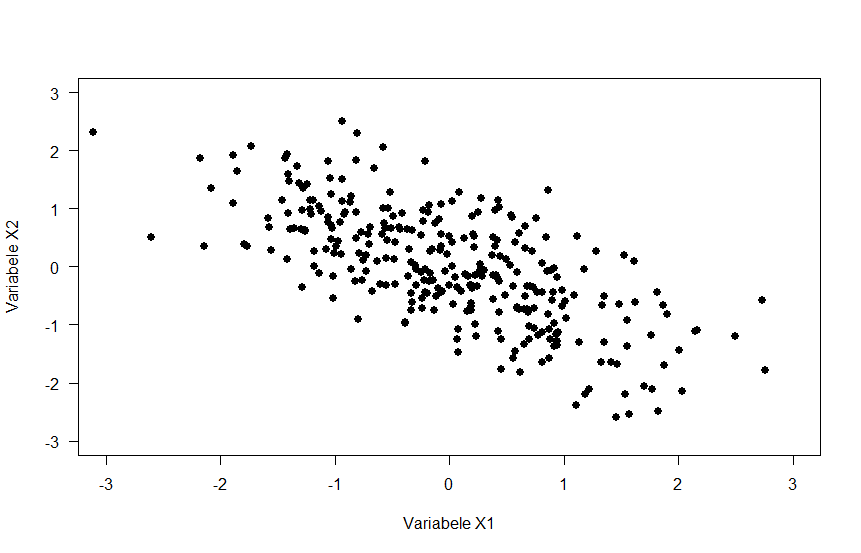
\includegraphics{images/lecture 73.png}\{width = 30\%\}

}

\end{minipage}%
%
\begin{minipage}[t]{0.33\linewidth}

{\centering 

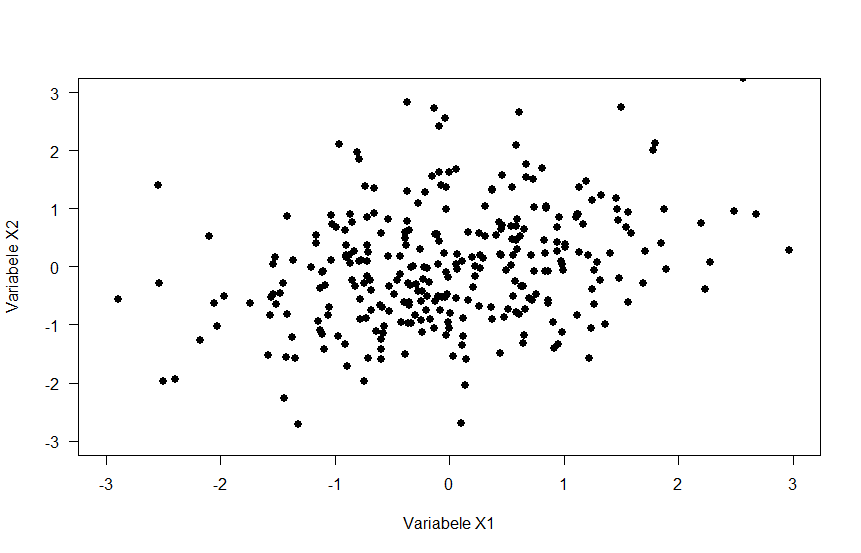
\includegraphics{images/lecture 74.png}\{width = 30\%\}

}

\end{minipage}%
%
\begin{minipage}[t]{0.33\linewidth}

{\centering 

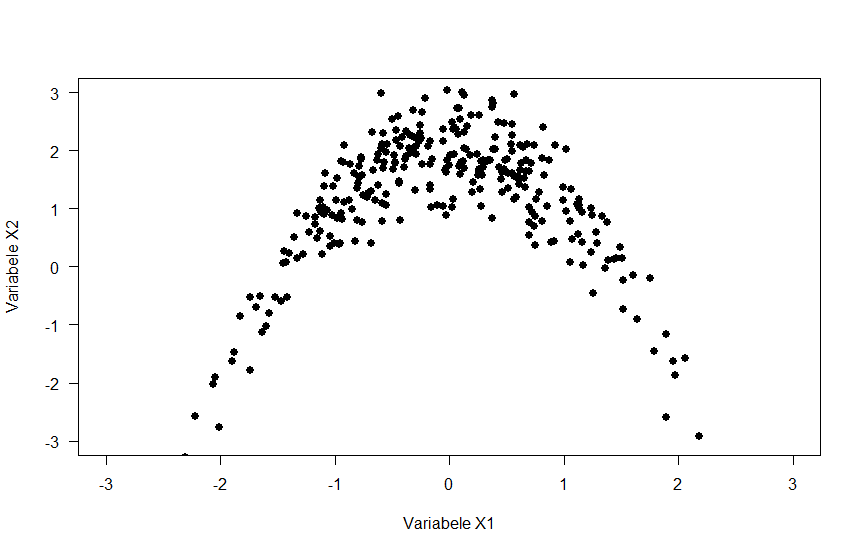
\includegraphics{images/lecture 76.png}\{width = 30\%\}

}

\end{minipage}%

\caption{\label{fig-scatter}Question 3 scatterplots}

\end{figure}

Six students work on a Statistics exam. They obtain the following
grades: 8, 9, 5, 6, 7 and 8. The teacher calculates a certain statistic,
which is equal to 7.5. Which statistic did the teacher calculate?

\begin{itemize}
\item
  \begin{enumerate}
  \def\labelenumi{(\Alph{enumi})}
  \tightlist
  \item
    Standard deviation\\
  \end{enumerate}
\item
  \begin{enumerate}
  \def\labelenumi{(\Alph{enumi})}
  \setcounter{enumi}{1}
  \tightlist
  \item
    Mode\\
  \end{enumerate}
\item
  \begin{enumerate}
  \def\labelenumi{(\Alph{enumi})}
  \setcounter{enumi}{2}
  \tightlist
  \item
    Median\\
  \end{enumerate}
\item
  \begin{enumerate}
  \def\labelenumi{(\Alph{enumi})}
  \setcounter{enumi}{3}
  \tightlist
  \item
    Mean\\
  \end{enumerate}
\end{itemize}

Show answers

\textbf{Question 1}

The variance is the sum of squared distances of observations to the
mean, divided by the number of observations minus one. So calculate:

\(S_{X}^2= \frac{\sum_{i=1}^nX_i}{n} = \frac{(7 + 6 + 8 + 6 + 8)}{5} = 7\)

\textbf{Question 2}

First rule out improbable answers; all grades are pretty close to each
other, so it's impossible for the variance to be that high. We can see
what the mode (most common value) is: it's 8. So we only choose between
mean or median.

Mean: calculate
\(\bar{X}= \frac{\sum_{i=1}^nX_i}{n} = \frac{8 + 9 + 5 + 6 + 7 + 8}{6} = 7.17\)

Median: order the numbers, note that there is an odd number, take the
average of the two middle numbers. 5, 6, 7, 8, 8, 9 -\textgreater{} 7.5

\textbf{Question 3}

Correlation measures linear association, so eliminate option C. Option B
shows a very small correlation - probably 0 or maybe .1. So the correct
answer is A, which shows a moderate negative correlation.

\bookmarksetup{startatroot}

\hypertarget{sec-probability}{%
\chapter{Probability Distributions}\label{sec-probability}}

Probability Distributions

Probability refers to the likelihood or chance of an outcome occurring
in a random experiment. It is defined as the proportion of times that a
particular outcome is expected to occur if the experiment is repeated an
infinite number of times.

A random experiment is a process with multiple potential outcomes that
could theoretically be repeated under similar conditions. For example,
flipping a coin is a random experiment, and before flipping the coin,
the outcome is a random experiment with a probability of getting heads
or tails of 50\% each. Once the coin is flipped, the outcome becomes
fixed (the opposite of random), resulting in either heads or tails.

In a way, when you draw samples from a population and observe the values
of particular variables (e.g., country of origin, height, age), you are
performing random experiments. That means that, like with any random
experiment, the values you are likely to observe also follow certain
probability distributions. Discrete random variables have a finite or
countable number of possible outcomes, such as the outcome of a coin
toss. On the other hand, continuous random variables, such as the height
of individuals, have an infinite number of possible outcomes.

For discrete (categorical) variables, we use discrete frequency and
probability distributions, which summarize the observations and
probabilities of each possible outcome, respectively. These
distributions can be represented using frequency distributions,
contingency tables, or bar charts.

Frequency distributions summarize observed outcomes in a sample. For
example, a frequency distribution can tell us the proportion of Dutch
students in a class or the number of times a particular number was
rolled on a die.

Contingency tables (also called crosstables) are used to describe the
join frequency distribution, and possibly relationship, between two
categorical variables. They show the frequencies of different
combinations of values for the two variables.

We can use frequency distributions to estimate the probabilities of
observing those outcomes in the future. To calculate probabilities from
frequencies, we can use different approaches depending on the type of
probability distribution we want. In general, dividing frequencies by
the total number of observations (grand total) gives us probabilities.
In contingency tables, marginal probability distributions are obtained
by dividing the marginal totals (row sums or column sums) by the grand
total, which provides us with a probability distribution for each
separate variable. Conditional probability distributions are derived by
dividing a specific row or column by the row- or column total (marginal
total), and tells us the probabilities of one variable given a specific
value of the other variable.

In continuous probability distributions, the possible outcomes are
infinite and described by a continuous function. One common example is
the normal distribution, also known as the bell curve. It is a symmetric
distribution that extends from negative infinity to positive infinity,
and it is characterized by two parameters: its mean (average) and
standard deviation (measure of dispersion). The square of the standard
deviation is called the variance.

The \emph{standard} normal distribution, also known as the
Z-distribution, is a standardized version of the normal distribution,
rescaled to have a mean of 0 and a standard deviation of 1.
Standardizing normal distributions allows us to calculate probabilities
more easily using standard normal distribution tables or calculators. We
can then convert these probabilities back to the original units if
needed.

Probability distributions can be used as models to describe/approximate
the distribution of real data. Behind the scenes, we do this any time we
describe the distribution of scores on a variable using its mean and
standard deviation. While we often assumpe that variables are normally
distributed, that assumption is not always accurate. For example,
depression symptoms do not follow a normal distribution: Most people
score near-zero on depression symptoms, and few people have higher
scores (but these are also not normally distributed). In such cases of
violations of the assumption of normality, the mean and standard
deviation are not very informative. You may use other descriptive
statistics, consider different probability distributions (outside the
scope of this course), or discuss the limitations of the assumption of
normality.

In conclusion, probability distributions provide a way to represent the
probabilities associated with different outcomes of a random variable,
whether discrete or continuous. By using probability distributions, we
can report descriptive statistics, calculate probabilities, and make
predictions about future observations.

\bookmarksetup{startatroot}

\hypertarget{sec-sampdist}{%
\chapter{The Sampling Distribution}\label{sec-sampdist}}

As explained in lecture 1, a sample is an observed subset of a larger
population. We typically calculate statistics based on sample data, and
use these as best guesses of the values of population parameters. This
process is called statistical inference. A crucial insight is that
sample statistics are not perfect estimates of population parameters.
The discrepancy between the sample statistic and population parameter is
known as sampling error.

We have some theoretical insight into theoretical behavior of sample
statistics. For example, we can imagine constructing a probability
distribution of the values we might see for a sample statistic, such as
the mean, if we were to draw very many random samples from an identical
population. This theoretical distribution of means is called the
sampling distribution. The central limit theorem tells us that,
regardless of the shape of the distribution of the data in the
population, as the sample size increases, the sampling distribution of
the mean approaches a normal distribution. This is an important
realization, because it means that we can use probability calculus using
the normal distribution to draw inferences about population parameters
based on sample statistics.

The standard deviation of the sampling distribution plays a central role
in inferential statistics. It is so important that we give it a unique
name: we call this particular standard deviation the \emph{standard
error} (SE). The standard error quantifies the average, or expected,
amount of sampling error when we use a sample statistic to estimate the
population parameter. If the standard error is small, our estimates
based on the sample are likely to be accurate, whereas a large standard
error indicates greater uncertainty.

With the help of the normal distribution, and given a particular
(hypothesized or known) population mean and standard error, we can
calculate how likely it is to observe specific sample means. For
example, if we want to determine the probability that the mean of a
random sample exceeds a certain value, we can standardize the sample
mean using the formula \$Z = \frac{M - \mu}{SE_M}, where M is the sample
mean, \(\mu\) is the known or hypothesized population mean, and SE is
the standard error. By looking up the corresponding probability on the
standard normal distribution table or using statistical software, we can
assess the likelihood of observing a specific sample mean (or greater,
or smaller).

Confidence intervals are a way to express our uncertainty about the
sample statistic as estimator of the population parameter. A confidence
interval is a range of values - a window - within which we expect the
true population parameter to fall with a certain level of confidence.
Typically, we select a 95\% confidence interval, which means that if we
could repeat the sampling process many times and calculated confidence
intervals each time, 95\% of those intervals would contain the true
population parameter. The width of the confidence interval is determined
by the standard error and is proportional to the level of confidence
desired. The formula for a confidence interval is often written as:
\(M \pm Z_{95%} * SE_M
\). In practice, this comes down to approximately: \(M \pm 2 * SE_M\).

\bookmarksetup{startatroot}

\hypertarget{sec-glm1}{%
\chapter{GLM-I: Linear Regression}\label{sec-glm1}}

The General Linear Model (GLM) is a family of models used to analyze the
relationship between an outcome variable and one or more predictors. In
this lecture, we will focus on bivariate linear regression, which
describes a linear relationship between a continuous outcome variable
and a continuous predictor. However, it's important to note that the GLM
encompasses other members that can handle predictors of any measurement
level (continuous or categorical), multiple predictors, transformations
of the outcome and predictors, and different error distributions.

Linear regression is based on the concept of using information about
other variables associated with the outcome to improve predictions. It
begins with the understanding that the mean is the best predictor
(expected value) when no further relevant information is available.
However, if we have information about other variables, such as the
number of hours studied being strongly associated with exam grades, we
can use that information to enhance our predictions. This process is
known as regression.

To visually explore associations between two variables, we often use
scatterplots. Scatterplots require both variables to be at least of
ordinal measurement level. By plotting the data points, we can observe
whether there is a linear pattern or trend. In linear regression, we aim
to find a line that represents the best possible predictions. This line,
called the regression line, goes through the middle of the cloud of data
points.

The regression line is described by the formula Y = a + bX, where ``a''
is the intercept (the predicted value when X equals 0) and ``b'' is the
slope (how steeply the line increases or decreases). The predictions
made using the regression line are not identical to the observed values,
as there is always some prediction error. The Ordinary Least Squares
method is used to obtain the line that minimizes the sum of squared
prediction errors.

In a bivariate regression, the regression formula expands to include the
individual prediction error, assuming that the errors are normally
distributed around the regression line with a mean of zero. The
regression model is represented as Yi = a + b * Xi + ei, where Yi is the
individual's score on the dependent variable, a is the intercept, b is
the slope, Xi is the individual's score on the independent variable, and
ei is the individual prediction error.

Hypothesis tests can be conducted on the regression coefficients to
determine their significance. The default null hypothesis for the
intercept is that it is equal to zero, while the null hypothesis for the
slope is also zero. The t-test is commonly used, with the degrees of
freedom being n - p, where n is the sample size and p is the number of
parameters. By testing the coefficients, we can determine the
statistical significance of the relationship between the predictor and
the outcome.

While linear regression offers valuable insights, it is essential to
consider the assumptions underlying the model. These assumptions include
linearity of the relationship between the predictor and the outcome,
normality of residuals (prediction errors), homoscedasticity (equal
variance of residuals), and independence of observations. Violations of
these assumptions can affect the validity of the model and lead to
misleading results. Checking and addressing these assumptions is crucial
for accurate and reliable regression analysis.

Linear regression is a powerful tool for analyzing the relationship
between variables, and a building block for many more advanced analysis
techniques. It allows us to make predictions based on available
information and understand the strength and significance of the
relationship between a continuous predictor and continuous outcome. By
considering the assumptions and conducting hypothesis tests, we can
ensure the validity of our regression models and draw meaningful
conclusions from the analysis.

\cleardoublepage
\phantomsection
\addcontentsline{toc}{part}{Appendices}
\appendix

\hypertarget{references}{%
\chapter*{References}\label{references}}
\addcontentsline{toc}{chapter}{References}

\markboth{References}{References}

\hypertarget{refs}{}
\begin{CSLReferences}{0}{0}
\end{CSLReferences}


\backmatter

\end{document}
